\documentclass[11pt]{article}
\usepackage{graphicx}
\usepackage[export]{adjustbox}
\usepackage{float}
\usepackage{listings}
\usepackage{amsmath}
\usepackage{color}
\definecolor{lightgray}{gray}{0.9}
\title{Final Value Theorem}
\date{2018\\ March}
\author{Nail Tosun - 2094563 -Section 5\\ Electric and Electronic Engineering Departmant, METU}
\begin{document}
\maketitle
\section*{Introduction}
Final Value Theorem is a mathematical property which can helps to determine $t=\infty$ values which can be useful for engineering purposes like steady state calculations.
\section*{Proof}
From derivative property of Laplace transform;
$$sX(s)=\int_{0^{-}}^{\infty}x'(t)e^{-st}dt \> + x(0^-) $$
Taking limit s goes to zero both side;
$$ \lim_{s\to 0} sX(s)=\lim_{s\to 0}\int_{0^-}^{\infty}x'(t)e^{-st}dt \> + x(0^-)$$
$$ \lim_{s\to 0} sX(s)=\int_{0^-}^{\infty}x'(t)e^{-0t}dt \> + x(0^-)$$
$$ \lim_{s\to 0} sX(s)=x(\infty)-x(0^-)+x(0^-)$$
$$ \lim_{s\to 0} sX(s)=x(\infty)$$
\subsection*{Conditions for proof}
\subsubsection*{There is a pole or poles at RHP}
We can't use final value theorem for that has unstable pole. For example $T(s)=\frac{1}{s-5}$ is a plant with unity feedback. We know that since we have positive pole time response has positive exponential and become infinite when t goes to infinite However;
$$\lim_{s\to 0}\frac{s}{s-5}=x(\infty)=0$$
Final value theorem gives us wrong answer. Then we can not use in this region.
\subsubsection*{Poles at the Imaginary axis}
We know that when the system has poles at the imaginary axis time response is oscillatory. Then final value of oscillatory function is meaningless. For example $T(s)=\frac{1}{s^2+4}$; 
$$\lim_{s\to 0}\frac{s}{s^2+4}=x(\infty)=0$$
Zero is the average final value of the system however, still final value theorem meaningless at that region. 
\subsubsection*{Poles at LHP}
$$T(s)=\frac{1}{s+5}$$
$$\lim_{s\to 0}\frac{s}{s+5}=x(\infty)=0$$
Which is true for system has negative poles. 
\subsubsection*{Poles at the origin}
$$T(s)=\frac{1}{s}$$
$$\lim_{s\to 0}\frac{s}{s}=x(\infty)=1$$
Which is make sense since time response for transfer function is 1.
\section*{System Types and Error Coefficients}
System types is the number of poles of the origin.
\subsection*{Type 0 System}
There is no integrator term in the system. All poles at the left half plane. For example;
$$G(s)=\frac{1}{s^2+6s+8}$$
\begin{figure}[H]
\centering
  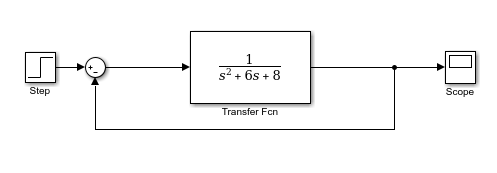
\includegraphics[scale=1]{type0}
  \caption{Type 0 system}
  \label{fig:zero}
\end{figure}
\begin{figure}[H]
\centering
  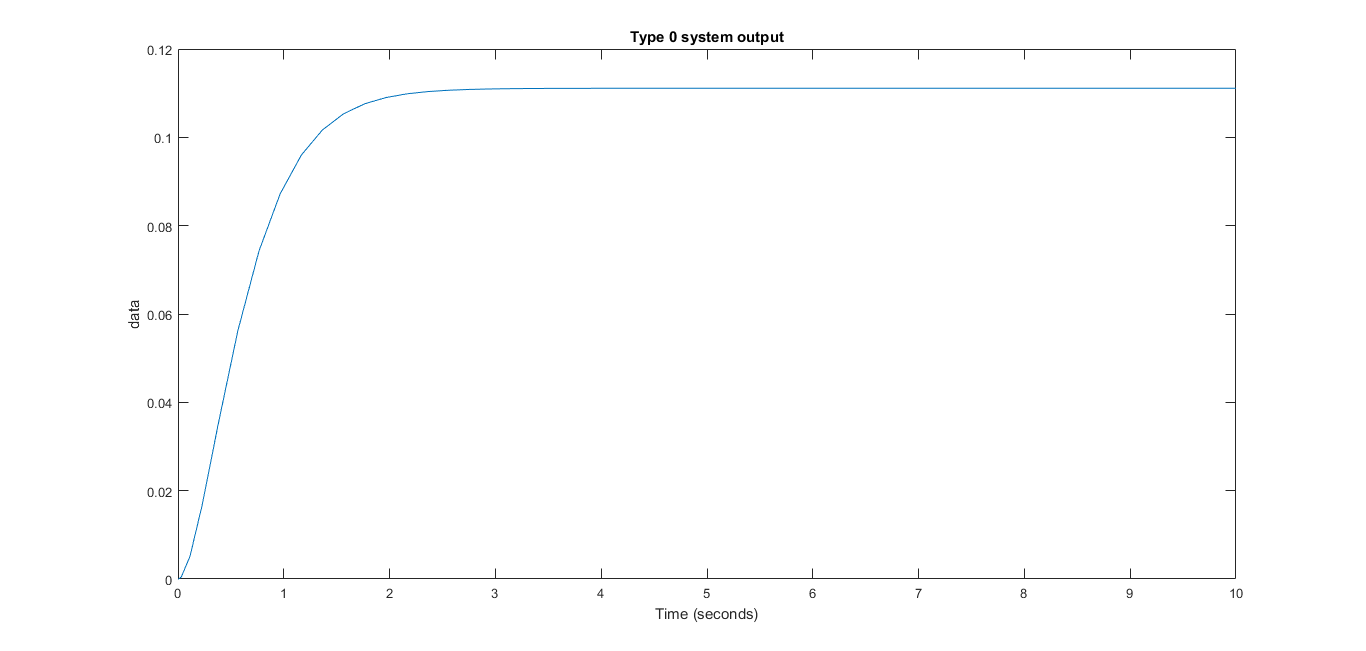
\includegraphics[scale=0.35]{type0response}
  \caption{Type 0 system response to step input}
  \label{fig:zero}
\end{figure}

\subsubsection*{Position Error Coefficient $K_d$}
Position error occurs when we give step input to the system. Type 0 systems has finite position error. 
$$K_p=lim_{x \to 0}G(s)H(s)=\frac{1}{s^2+6s+8}=\frac{1}{8}$$
$$e_{ss}=\frac{1}{1+K_p}=\frac{8}{9}$$
\subsection*{Type 1 system}
There is one integrator term occur in the transfer function. Type one system has no position steady state error.(Or we can say $K_p=\infty$). However it has finite velocity error. Velocity error occurs when we give ramp input to the system. 
\begin{figure}[H]
\centering
  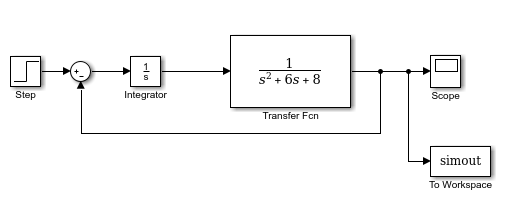
\includegraphics[scale=1]{type1}
  \caption{Type 1 system}
  \label{fig:zero}
\end{figure}
Now G(s)H(s) has one integrator term then it is Type 1 system. Adding integrator to type 0 system can be used as improving position error of the system. Following figure we can see effect of the adding integrator to the type 0 system.
\begin{figure}[H]
\centering
  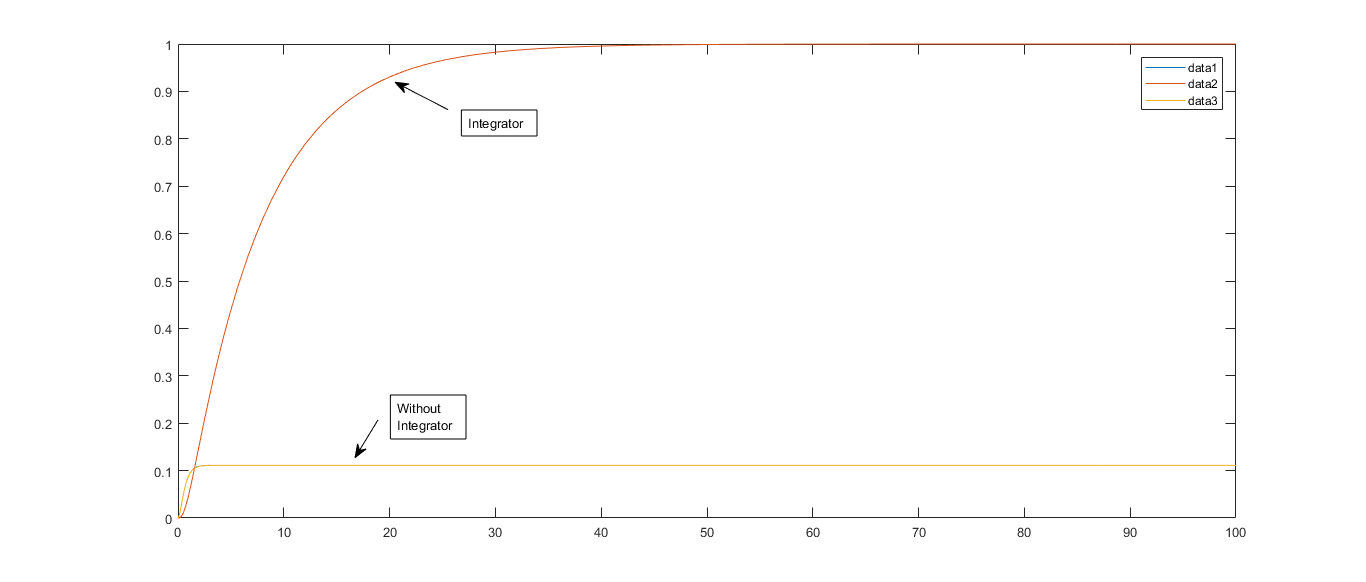
\includegraphics[scale=0.4]{compare}
  \caption{Comparing type 1 and type 0 time response}
  \label{fig:zero}
\end{figure}

\end{document}